\documentclass[11pt]{article}
\usepackage[utf8]{inputenc}
\usepackage[french]{babel}
\usepackage{graphicx}
\usepackage[T1]{fontenc}
\usepackage{amsmath}
\usepackage{amsfonts}
\usepackage{amssymb}
\def\N{\mathbb N}
\def\R{\mathbb R}
\def\Q{\mathbb Q}
\def\Z{\mathbb Z}
\begin{document}
\title{EXAMEN ALGORITHMIQUE AVANCEE}
\author{LICENCE 2, MODULE I31}
\date{18 décembre 2014} 
\maketitle
\newif\ifcorrige
\corrigetrue
%\corrigefalse

\newcommand{\smallbullet}{\,\begin{picture}(-1,1)(-1,-3)\circle*{2}\end{picture}\ }

\fbox{\parbox{0.95\linewidth}{LA COPIE EST NOTEE ZERO DES QU'IL Y A UN PROGRAMME.}}

\bigskip

\section{La méthode de Newton}

1. La fonction $f$ est définie par $f(x)=x^2-4$. Donnez $f'(x)$.

2. Donnez  $N(x)$, où $N$ est la fonction de Newton associée.
Expliquez à quoi elle sert, en 2 lignes au plus.

3. Donnez $N'(x)$.

4. Calculez (à la main ou avec une calculette) $N(1/2), N(1), N(2), N(3), N(4)$ et dessinez  approximativement, mais avec soin, la courbe $(x, N(x))$ pour $1/2 \le x \le 4$.
Dessinez aussi la droite d'équation $y=x$.
En partant de $x_0=4$, donnez les valeurs de $x_k= N(x_{k-1})$ pour $k=1$ à 3 et
dessinez le "trajet" correspondant sur la courbe, comme vous l'avez vu en cours.

\section{L'erreur d'Arthur}

Arthur a programmé le dessin du fractal de Sierpinski.
Pour tracer le triangle de Sierpinski de  trois points donnés $(A, B, C)$ au
niveau de récursion $n$,
Arthur remplit le triangle $ABC$, et quand $n$ est plus grand que 0, il 
trace récursivement trois triangles de Sierpinski  au niveau $n-1$, qui sont~: $(A, B', C')$,
$(B, A', C')$ et $(C, A', B')$ où $A'$ est le milieu de $BC$, $B'$ celui de $AC$ et $C'$ celui de $AB$. 

Que voit Arthur sur son dessin, à sa grande déception~?
Quelle est son erreur~? 

{
\section{Les ensembles non consécutifs}
Un ensemble d'entiers est dit non consécutif s'il ne contient pas deux entiers consécutifs ($n$ et $n+1$ sont consécutifs, pour $n\in \N$). 
Par définition, $F_k$ est l'ensemble des sous-ensembles  non consécutifs d'entiers dans l'intervalle $[1 \ldots k]$ (zéro est inutilisé, pour simplifier). 

On note $f_k$ le nombre d'éléments (de sous ensembles) de $F_k$. Rappelons que $\emptyset$ est l'ensemble vide. Ce dernier ne contient rien (même pas zéro).

Par exemple~: \\
\indent $F_0=\{ \emptyset \}$,  $f_0=1 $, \\
\indent $F_1= \{ \emptyset, \{1\}\}$, $f_1= 2$,\\
\indent $F_2= \{ \emptyset, \{1\}, \{2\} \}$, $f_2=3$,\\
\indent $F_3= \{ \emptyset, \{1\}, \{2\}, \{3\}, \{1, 3\}\}$, $f_3=5 $,\\
\indent $F_4= \{ \emptyset, \{1\}, \{2\}, \{3\}, \{4\},  \{1, 3\}, \{1, 4\}, \{2, 4 \}\}$, $f_4=8$.

Définissons~:
$$F_k \oplus v= \bigcup_{E\in F_k} \{v\} \cup E$$ 

Par exemple, 
$$F_2 \oplus 4= \{ \{4\}, \{1,4\},  \{2, 4\}  \}$$

1. Quel est le plus petit entier $v\in \N$ qui assure que  $F_k \oplus v$ est un ensemble non consécutif~?

\ifcorrige

\medskip
{\it  Réponse.
$v \ge k+2$
}
\medskip

\else
\fi

2. Calculez $(F_1 \oplus 3) \cup F_2$.
Comparez avec $F_3$.
Calculez $(F_2 \oplus 4)  \cup F_3$.
Comparez avec $F_4$.
Que constatez-vous~?

3.
En généralisant pour tout  $k\ge 2$, conjecturez une  définition récursive de $F_k$ en fonction de $F_{k-1}$ et $F_{k-2}$.
Aucune preuve n'est demandée (mais donnez une conjecture exacte!).


\ifcorrige

\medskip

{\it  Réponse.
$F_0= \{ \emptyset \}$, $F_1= \{ \emptyset, \{1\}\}$ et pour  $k>1$~:
$F_k= F_{k-1} \cup (F_{k-2}\cup k)$;
}
\medskip


\else
\fi

4. En déduire une formule récursive pour $f_k$.

\ifcorrige

\medskip

{\it  Réponse.
$f_0=1, f_1=2, f_k= f_{k-1} + f_{k-2}$.
}
\medskip


\else
\fi

5. Reconnaissez vous $f_k$~? Si oui, qui est $f_k$~?

\ifcorrige

\medskip

{\it  Réponse.
C'est la suite de Fibonacci, décalée.
}
\medskip


\else
\fi 
}

{
\section{Algorithme d'Euclide}
Utilisez  l'algorithme d'Euclide généralisé
pour calculer le PGCD $g$ de $a=210$ et $b=66$. Outre le PGCD, vous devez
aussi calculer deux entiers relatifs $u$ et $v$ tels que $a u + b v=g$.
Utilisez une présentation sous forme de tableau, comme en TD.
}

{
\section{Matrices}
Soient $A$ et $B$ deux matrices données. $A$ a $l_A$ lignes et $c_A$ colonnes.
$B$ a $l_B$ lignes et $c_B$ colonnes. Soit $M= A B$. La matrice $M$ a $l_M$ lignes et $c_M$ colonnes. 

1. Définissez $l_M$ et $c_M$ en fonction de $l_A, c_A, l_B, c_B$. Y-a-t-il des
contraintes  sur $l_A, c_A, l_B, c_B$
pour que le produit $AB$ soit possible~? Si oui, lesquelles~? (il est inutile de mentionner que  $l_A, c_A, l_B, c_B$ sont des entiers de $\N$).  

\ifcorrige

\medskip
{\it 
Réponse. $M$ a $a$ lignes et $b'$ colonnes. $M_{lc}$ est le produit scalaire
de la ligne $l$ de $A$ par la colonne $c$ de $B$; Il faut donc que $a'=b$. 
}
\medskip


\else
\fi

2. Définissez $M_{l,c}$ (ou $M[l][c]$ en Java ou en C), pour que $M=AB$,
par une formule avec un signe $\sum$ (les indices commencent à 0; $l$ est le numéro de ligne et $c$ le numéro de colonne).
Combien de multiplications (entre nombres flottants) sont nécessaires pour calculer  $M_{l,c}$~?

\ifcorrige

\medskip
{\it 
Réponse. $$M_{l,c}= \sum_{k=0}^{b-1} A_{l,k} B_{k,c} $$
Il y a $b=a'$ multiplications pour calculer $M_{l,c}$.
}
\medskip


\else
\fi


{
3.  Calculez~:
$$\left( 1 \quad 2\right) \left(\begin{array}{c} 3\\
4
\end{array}\right) $$


{
\ifcorrige

\medskip
{\it

Réponse. C'est la matrice (11), ou le vecteur (11), ou bien le nombre 11. Cet abus de langage est consacré par l'usage. 
}
\medskip

\else
\fi
}

4. Calculez~:
$$\left(\begin{array}{c} 1 \\
2
\end{array}\right) \left( 3\quad 4\right) $$

\ifcorrige

\medskip

{\it C'est la matrice $$\left(\begin{array}{cc} 3 & 4 \\
6 & 8 \end{array}\right)$$
}
\medskip


\else
\fi
}
\bigskip
}
{
\section{Algorithme d'Euclide matriciel}
Une autre méthode  de calcul du PGCD de $a$ et $b$ utilise des matrices, dites d'Euclide~:
$$
\left( \begin{array}{c} a \\
b\end{array}\right) = \left( \begin{array}{cc} q & 1\\
1 & 0 \end{array}\right) \left( \begin{array}{c} b\\
r \end{array}\right) \mbox{ pour } a = bq + r \mbox{ où }  q=\left\lfloor \frac{a}{b}\right\rfloor, r = a \mbox{ mod } b$$
Par exemple, pour $a=35$ et $b=10$~:
$$
\left( \begin{array}{c} 35 \\
10 \end{array}\right) = \left( \begin{array}{cc} 3 & 1 \\
1 & 0 \end{array}\right) \left( \begin{array}{c} 10\\
5 \end{array}\right)$$
Puis~:
$$
\left( \begin{array}{c} 10 \\
5  \end{array}\right) = \left( \begin{array}{cc} 2 & 1\\
1 & 0 \end{array}\right) \left( \begin{array}{c} 5 \\
0 \end{array}\right)$$
L'algorithme a terminé car le reste est nul.
Donc~:  
$$
\left( \begin{array}{c} 35 \\
10 \end{array}\right) = \left( \begin{array}{cc} 3 & 1 \\
1 & 0 \end{array}\right) \left( \begin{array}{cc} 2 & 1\\
1 & 0 \end{array}\right) \left( \begin{array}{c} 5 \\
0 \end{array}\right)= \left( \begin{array}{cc} 7 & 3\\
2 & 1 \end{array}\right) \left( \begin{array}{c} 5 \\
0 \end{array}\right)$$

La matrice carrée finale $M$  contient, dans sa colonne gauche, $\frac{a}{g}$ et $\frac{b}{g}$,
et dans sa colonne droite deux entiers $U$ et $V$ tels que
$|M|=\frac{a}{g} U - \frac{b}{g} V = \pm 1$. On a $|M|=\pm 1$
car  le déterminant de chaque matrice d'Euclide vaut -1, 
et le déterminant d'un produit de matrices 
est le produit des déterminants des matrices. On  déduit de~: $aU-bV= \pm g$ les deux nombres de Bézout $u$ et $v$ pour $a$ et $b$;
$U$ et $u$ sont égaux au signe près, de même pour $V$ et $v$. 

Faites les calculs avec cette forme matricielle pour $a=210$, $b=66$.
Déduisez en le PGCD $g$ et les nombres de Bézout $u, v$ de $a$ et $b$, tels que
$au+bv=g$.
}







{
\section{Réseau}
{
\begin{figure}
\begin{center}
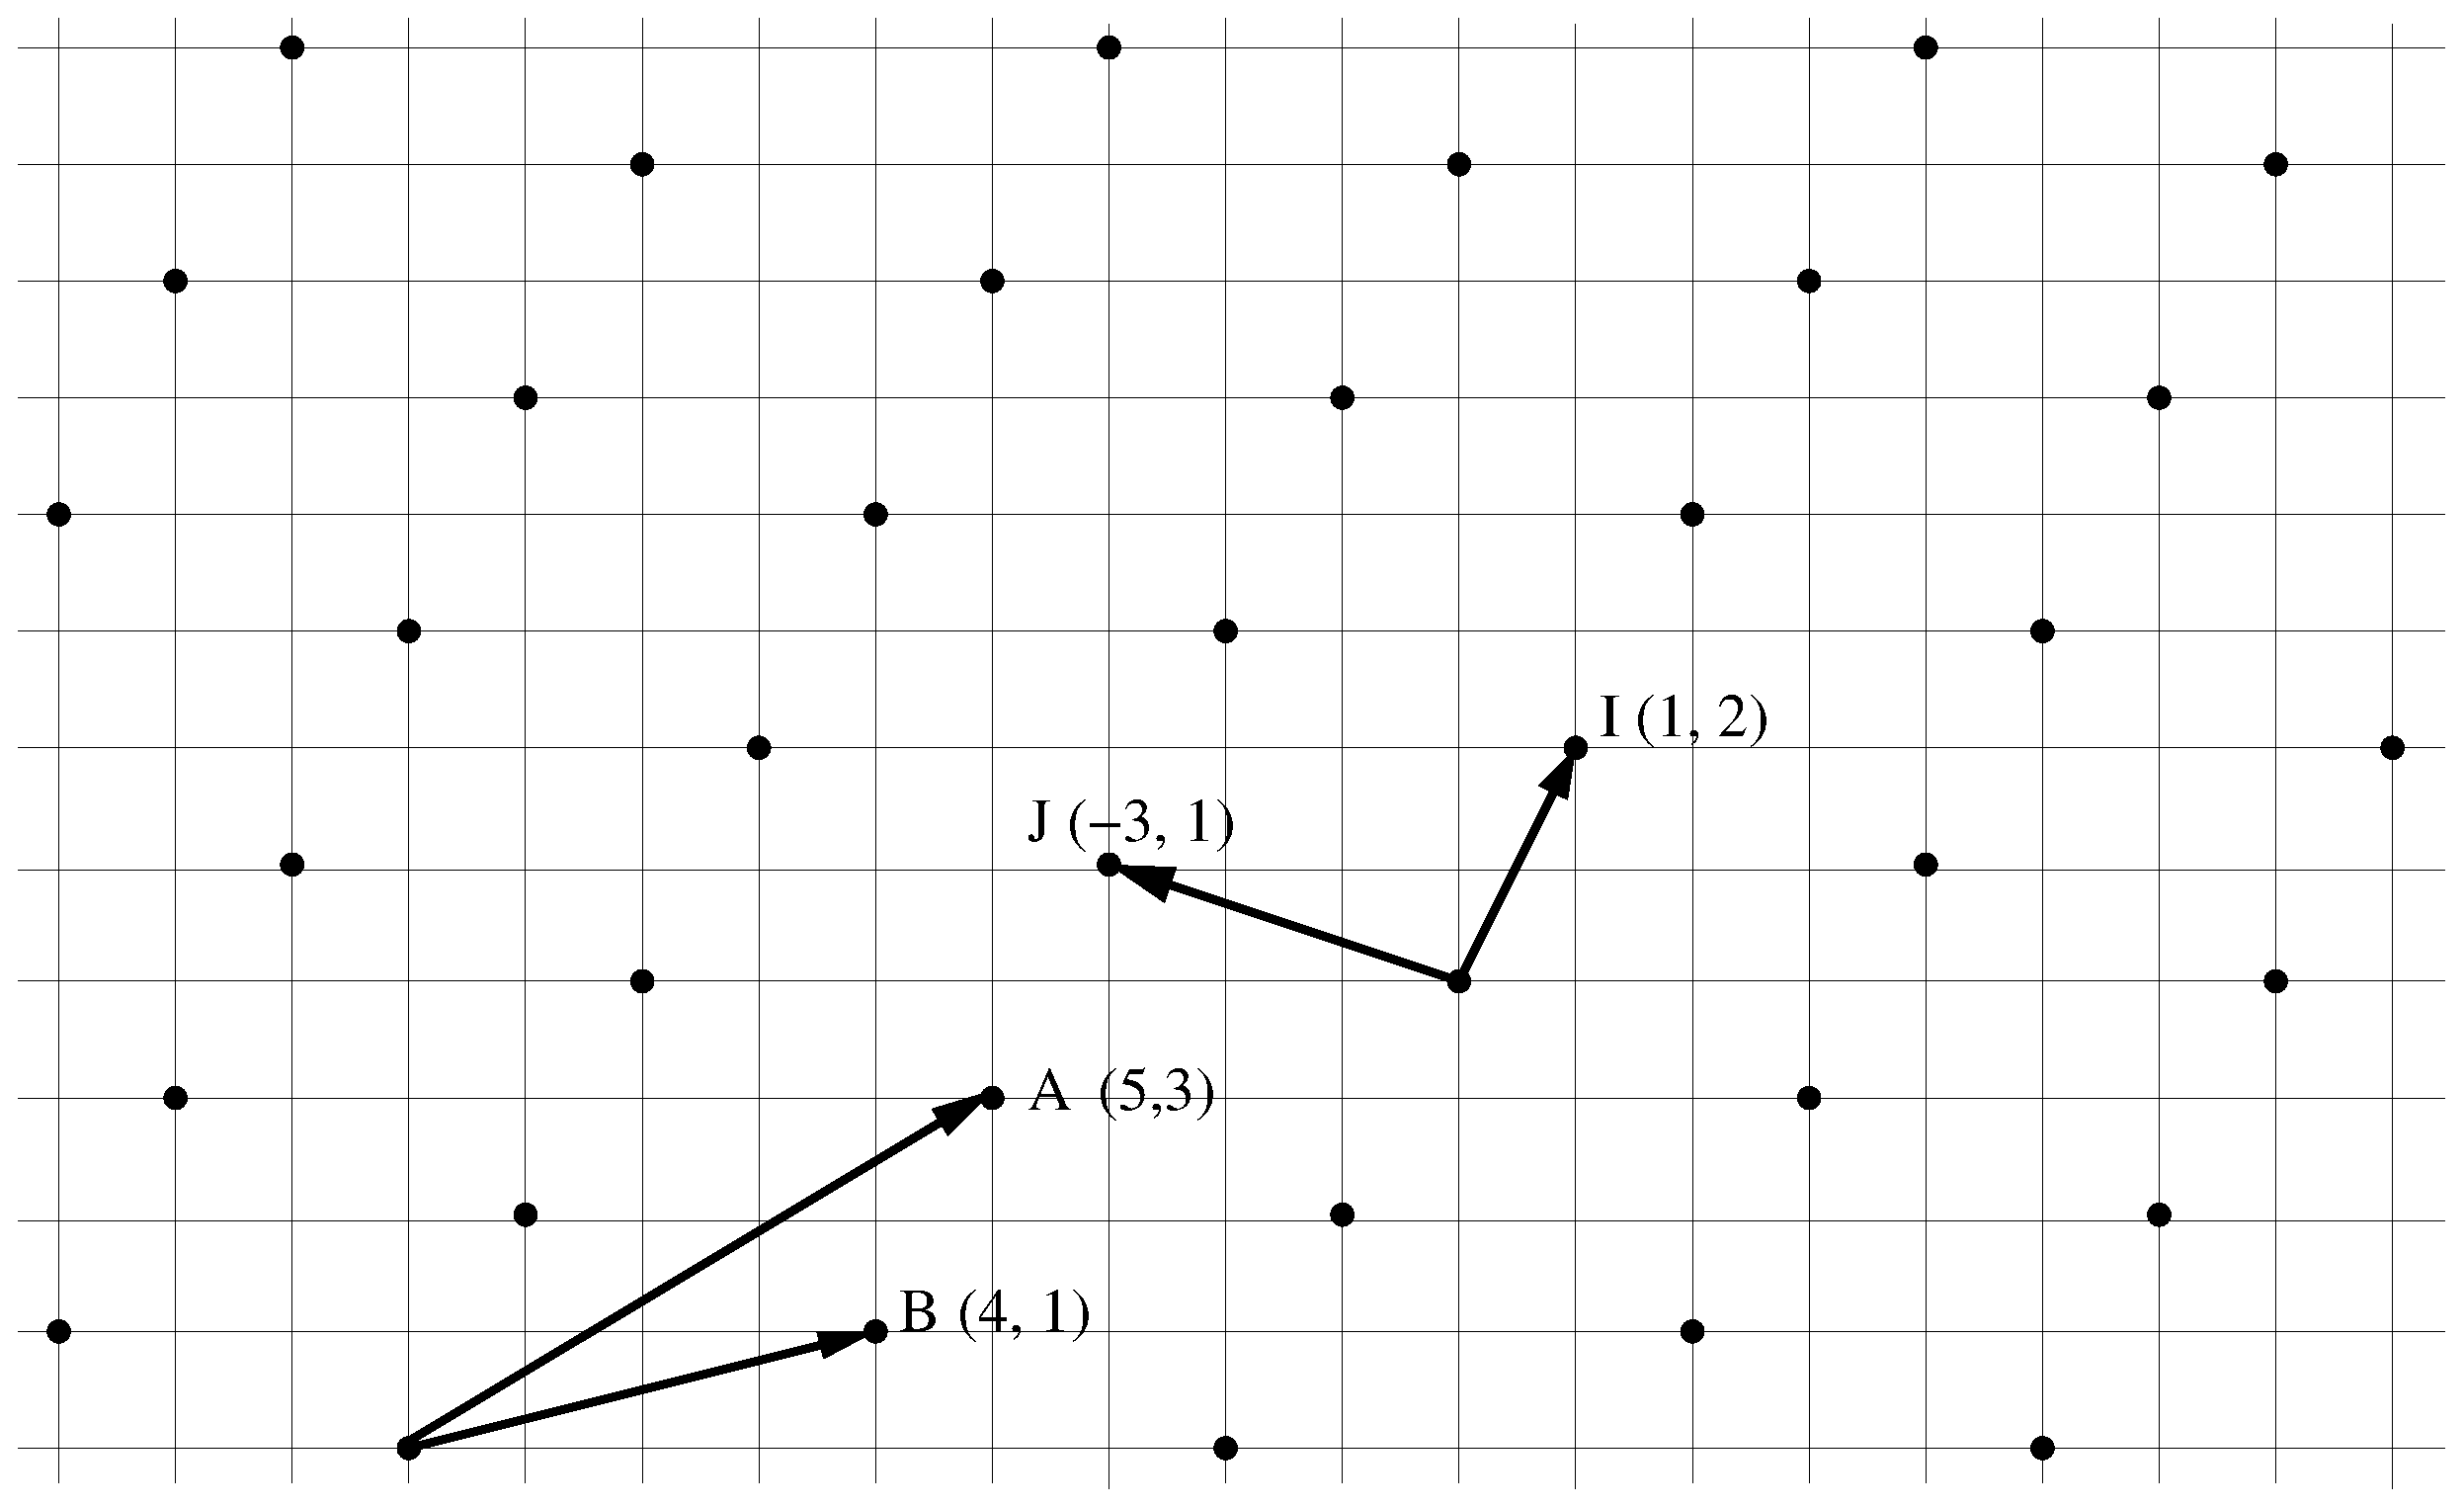
\includegraphics[width=0.99\linewidth]{dessin3.eps}
\end{center}

\caption{ Un réseau  généré par deux vecteurs $A$ et $B$. Le même réseau est  généré par $I, J$, plus courts que $A$ et $B$. }
\end{figure}
}
Ici, les vecteurs sont notés en ligne, par exemple~: $A=(5, 3)$.
Deux vecteurs $A$, $B$ donnés, à coordonnées dans $\Z$,
génèrent un réseau de points $aA + bB$, avec $a\in \Z, b\in\Z$. 
Ce réseau est parfois noté $\Z A + \Z B$.
Sur la figure ci-dessus, $A=(5, 3)$ et $B=(4, 1)$ et chaque disque noir  représente
un élément (un sommet, ou vecteur, ou point) du réseau. Le réseau est infini, et la figure n'en montre qu'une partie finie, dans un rectangle. 
Les
vecteurs  $I=(1, 2)$ et $J=(-3, 1)$ sont plus courts que $A$ et $B$, et génèrent le même réseau~: $\Z A + \Z B = \Z I + \Z J$. 
Il n'existe pas de vecteurs strictement plus courts que $\pm I, \pm J$ pour ce réseau. 

Rappel: la longueur, ou norme, d'un vecteur $v=(x, y)$ est $||v||=\sqrt{v \smallbullet v}=\sqrt{x^2+y^2}$.
Bien sûr, pour comparer deux longueurs, vous n'avez pas besoin d'extraire les racines carrées~: vous pouvez comparer les carrés des normes.


On peut calculer
deux vecteurs les plus courts 
par une variante de la méthode d'Euclide, que voici~:
on suppose que $A$ est plus long que $B$ (sinon, vous échangez $A$ et $B$).  Soit $R$ le vecteur le plus court parmi  les deux vecteurs~: 
$A + B$ et $A -B$.
Si $R$ n'est pas plus court que $A$, alors $(\pm A, \pm B)$ est la
paire la plus courte~; sinon l'algorithme recommence sur la paire $(B, R)$ ou $(R, B)$. 

1. Effectuez  les diverses étapes de cet algorithme sur l'exemple~:
$A=(5, 3)$, $B=(4,1)$, de normes respectives $\sqrt{34}$ et $\sqrt{17}$.


{
\ifcorrige

\medskip

{\it Réponse.
Algorithme 1: on suppose que $A$ est plus long que $B$;  soit $R$ le vecteur le plus court de  $A \pm B$. Si $R$ n'est pas plus court que $A$, alors $(A, B)$ est une paire la plus courte~; sinon on recommence sur la paire $(B, R)$ (ou bien $(R, B)$). 
Cette méthode est similaire à la méthode d'Euclide qui utilise la différence.
Voici les étapes:  \\

Etape 1: Les deux vecteurs de base sont $A=(5, 3), B=(4, 1)$. Le vecteur $A-B= (1, 2)$ est plus court que $A$ et le remplace. 

Etape 2: On échange les deux vecteurs de base, qui sont $A=(4, 1), B=(1, 2)$. Le vecteur  $A-B=(3, -1)$
est plus court que $A+B=(5, 3)$, et plus court que $A$ et le remplace.

Etape 3: Les deux vecteurs de base sont $A=(3,-1)$ et $B=(1, 2)$. Ni $A+B=(4,1)$, ni $A-B=(2, -3)$ ne sont plus courts que $A$. Donc la base la plus courte est $(3,-1)$ et $(1, 2)$.


\else
\fi

\medskip

}
}

{
2. Cet algorithme termine en un nombre fini d'étapes. Prouvez le (2 lignes au plus). 

{
\ifcorrige
\medskip

{\it Comme les tailles (les carrés des longueurs des vecteurs de la paire) sont des entiers de $\N$, et que chaque étape
diminue une des tailles, l'algorithme termine en un nombre fini d'étapes.
C'est différent de la convergence de la méthode de Newton, qui s'approche du point fixe mais ne l'atteint jamais.
}

\else
\fi
\medskip

}
}
{
\begin{figure}
\begin{center}
%%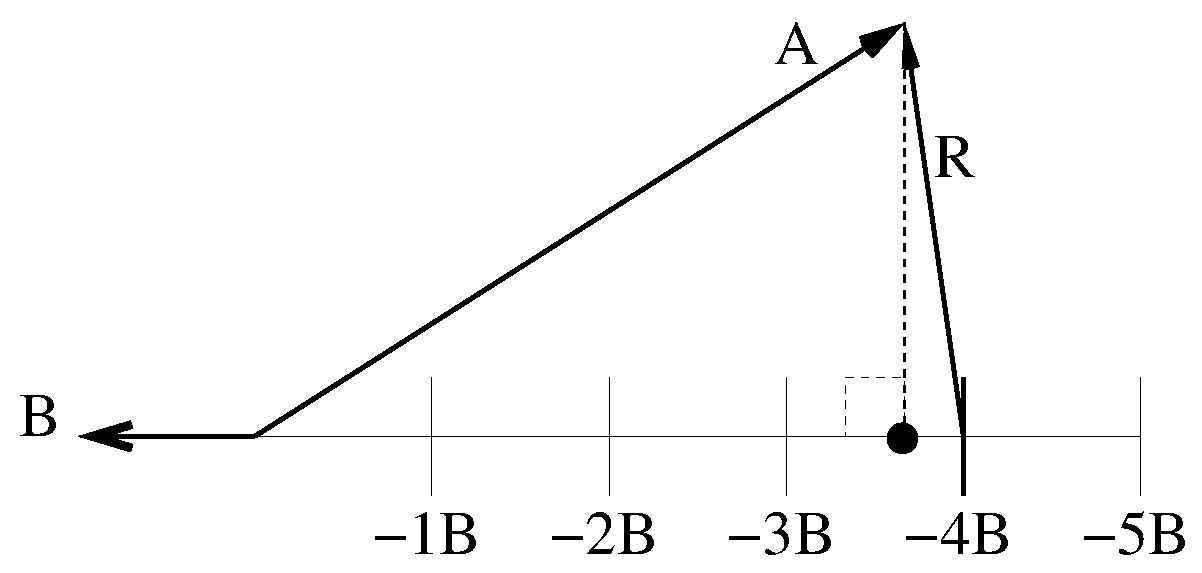
\includegraphics[width=0.5\linewidth]{projectionorthogonale.eps}
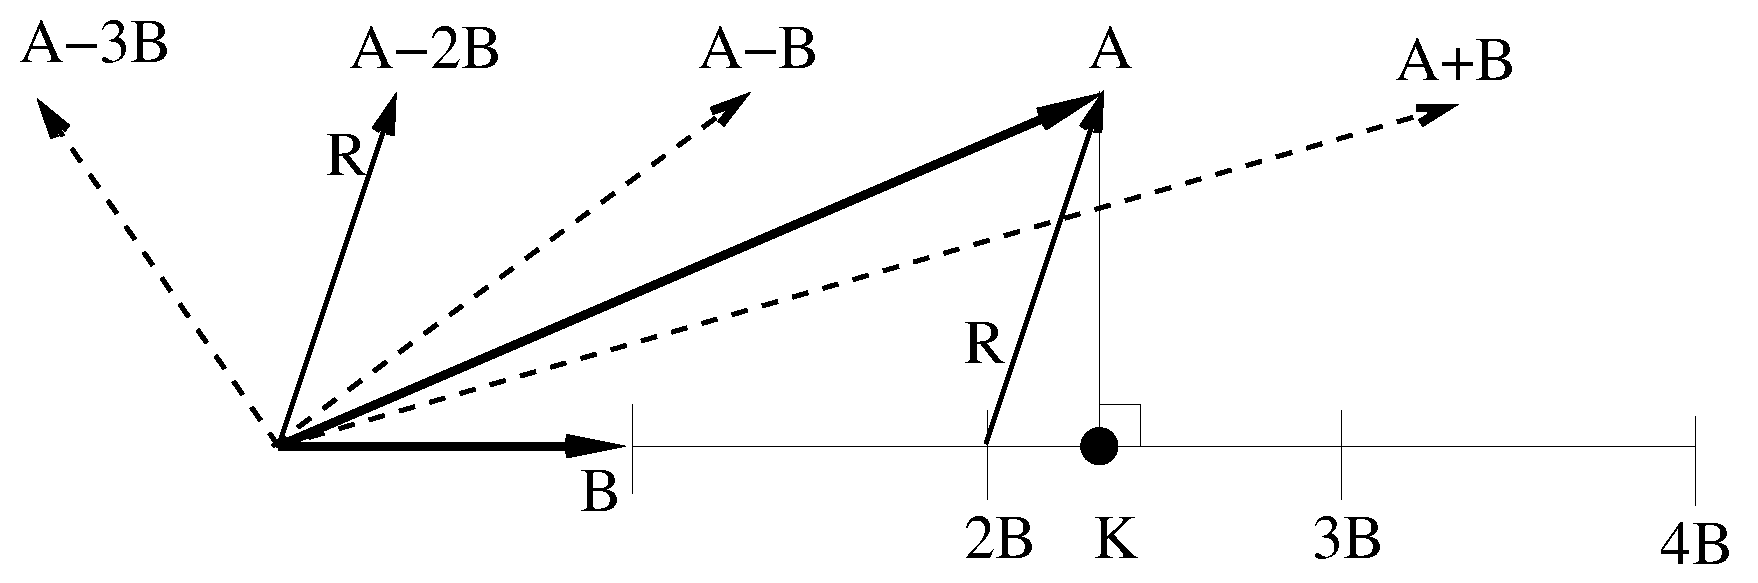
\includegraphics[width=0.8\linewidth]{porgo.eps}
\end{center}
\caption{\label{portho} Pour $A, B$ deux vecteurs donnés, on cherche le vecteur $R=A-qB$ le plus court, avec $q\in\Z$. La solution est obtenue en projetant orthogonalement l'extrémité de $A$ sur la droite supportée par $B$, en $K$,
puis en  arrondissant $K$ sur le  multiple entier de $B$ le plus proche, ici $2B$.}
\end{figure}
}

3. Pour accélérer la méthode précédente, nous allons calculer l'entier $q\in \Z$ qui minimise la taille du reste $R$ dans $A=qB+R \Rightarrow  R=A-qB$.
%(les noms $q$ pour quotient   et $R$ pour reste sont  choisis 
%par analogie avec 
%l'algorithme d'Euclide).
%%Que $q$ soit optimal signifie que le vecteur reste $R=A-qB$ est plus court
%%que les vecteurs $A-(q+1)B$ et $A-(q-1)B$.
Proposez une méthode ou une formule pour trouver la valeur optimale de $q$.
Vous pouvez vous inspirer de la figure \ref{portho}.

{
\ifcorrige

{
\medskip
{\it Algorithme 2: on calcule $Q\in \Z$ tel que $A-qB$ est le plus court possible. 
Soit $K$ la projection orthogonale de $A$ sur $B$; alors $K=\lambda B$, et
$q$ est l'entier le plus proche de $-\lambda$.  
Si 
$q=0$, alors $A, B$ est la paire la plus courte, sinon on recommence sur
$B, R=A-qB$.
Détaillons le calcul de $\lambda$. $(A-\lambda B) \smallbullet B=0 \Rightarrow \lambda=\frac{A \smallbullet B}{ B \smallbullet B}=\frac{A_x B_x + A_y B_y}{B_x^ 2 +B_y^ 2}$, et $q= - \lfloor \lambda \rfloor$.
Autre possibilité~: calculer $R$ pour $q= -1$ et $q=1$; en déduire le signe du $q$ optimal; trouver un encadrement de $q$ en considérant des puissances de 2 pour $q$; puis procéder par dichotomie dans l'intervalle des deux puissances consécutives de 2 qui contiennent le $q$ optimal.
}

\medskip
}
\else
\fi
}

4. On suppose  que $A$ est plus long que $B$, et
que $R=A-qB$ est plus court que $A$.
En notant $R=(R_x, R_y)$, $A=(A_x, A_y)$, et $B=(B_x, B_y)$, 
 écrivez l'équation~: $A=qB+R$ sous forme matricielle, avec des matrices de taille 2 par 2.
%par analogie avec la forme matricielle de l'algorithme d'Euclide.
Une matrice d'Euclide doit apparaître.


{
\ifcorrige

\medskip

{\it  Réponse.
$$\left( \begin{array}{cc} A_x & A_y \\
B_x & B_y \end{array}\right) = \left( \begin{array}{cc} q & 1 \\
1 & 0 \end{array}\right) \left( \begin{array}{cc}  B_x & B_y \\
R_x & R_y \end{array}\right)$$

On reconnaît la matrice de l'algorithme d'Euclide, celle qui contient $q$ et qui est de déterminant -1.

Voici les étapes pour l'algorithme 2 (Ceci n'était pas demandé dans l'examen).

$$\left( \begin{array}{cc} 5 & 3 \\
4 & 1 \end{array}\right) = \left( \begin{array}{cc} 1 & 1 \\
1 & 0  \end{array}\right)  \left( \begin{array}{cc}4 & 1 \\
1 & 2  \end{array}\right) \mbox{ car } \lambda=\frac{23}{17}, q=1 $$

$$\left( \begin{array}{cc} 4 & 1 \\
1 & 2 \end{array}\right) = \left( \begin{array}{cc} 1 & 1 \\
1 & 0  \end{array}\right) \left( \begin{array}{cc} 1 & 2 \\
3 & -1  \end{array}\right) \mbox{ car } \lambda=\frac{6}{5}, q=1 $$

$$\left( \begin{array}{cc} 1 & 2 \\
3 & -1 \end{array}\right) = \left( \begin{array}{cc} 0 & 1 \\
1 & 0  \end{array}\right) \left( \begin{array}{cc} 3 & -1 \\
1 & 2  \end{array}\right) \mbox{ car } \lambda=\frac{1}{10}, q=0 $$ Mais ce n'est pas fini bien que $q=0$, car $A$ est plus court que $B$. Cette étape permet donc d'échanger $A$ et $B$.

$$\left( \begin{array}{cc} 3 & -1 \\
1 & 2 \end{array}\right) = \left( \begin{array}{cc} 0 & 1 \\
1 & 0  \end{array}\right) \left( \begin{array}{cc} 1 & 2 \\
3 & -1  \end{array}\right) \mbox{ car } \lambda=\frac{1}{5}, q=0 $$ 

Ce coup ci, c'est terminé. $A$ est plus long que $B$, et $q=0$. Donc il est impossible de remplacer le plus long vecteur, $A$, par un plus court. 

Donc:
$$\left( \begin{array}{cc} 5 & 3 \\
4 & 1 \end{array}\right) = 
\left( \begin{array}{cc} 1 & 1 \\
1 & 0 \end{array}\right) 
\left( \begin{array}{cc} 1 & 1 \\
1 & 0  \end{array}\right)  
\left( \begin{array}{cc} 0 & 1 \\
1 & 0  \end{array}\right)  
\left( \begin{array}{cc} 0 & 1 \\
1 & 0  \end{array}\right)\left( \begin{array}{cc}  1 & 2 \\
3 & -1  \end{array}\right)$$

Après quelques calculs:
$$\left( \begin{array}{cc} 5 & 3 \\
4 & 1 \end{array}\right)   = \left( \begin{array}{cc} 2 & 1 \\
1 & 1 \end{array}\right)\left( \begin{array}{cc}  1 & 2 \\
3 & -1  \end{array}\right) $$ 

Les deux vecteurs les plus courts sont donc $I=(1, 2)$ et $J=(3, -1)$.
De plus les deux vecteurs initiaux de base sont $A=(5, 3) = 2 I + J$ et $B=(4, 1)= I + J$.
}
\medskip

\else
\fi
}



\end{document}

\bigskip
5. Décrivez en 5 lignes au plus  un algorithme (pas de programme~!) de recherche arborescente ({\it backtrack}) pour générer les
k! permutations de 1, 2, \ldots k. 


\Question{Citez les noms de 3 algorithmes de tri}
~\\
~\\

\Question{Citez les noms de 3 algorithmes calculant les plus courts chemins dans un graphe}
~\\
~\\




\Question{Donnez les formules n\'ecessaires pour le calcul r\'ecursif 
de $a^n$ ($a$ est une matrice carrée, à valeurs enti\`eres). N'oubliez pas le ou les cas terminaux}  


~\\
~\\
~\\
~\\
~\\

\begin{center}
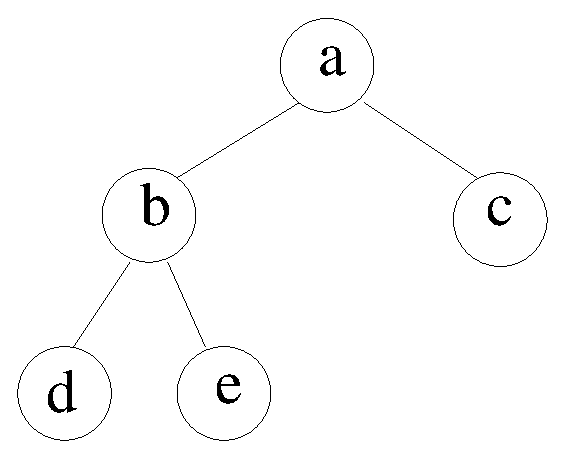
\includegraphics[width=0.7\linewidth]{arbrebin.eps}
\end{center}
\Question{Dans l'arbre ci-dessus, l'affichage: a, b, c, d, e est obtenu par}
\begin{Reponse}
\Vrai un parcours en largeur
\Faux un parcours en  profondeur
\end{Reponse}


\Question{Dans l'arbre ci-dessus, l'affichage: a, b, d, e, c est obtenu par}
\begin{Reponse}
\Faux un parcours en largeur
\Vrai un parcours en  profondeur
\end{Reponse}


\Question{Un algorithme optimal de tri,  n'utilisant que des comparaisons entre 2 \'el\'ements,
n\'ecessite}
 \begin{Reponse}
\Vrai $O(n \log n)$ comparaisons pour trier $n$ \'el\'ements
\Faux $O(n^2)$ comparaisons 
\Faux $O(n)$ comparaisons
\Faux un nombre exponentiel de comparaisons
\end{Reponse}


\Question{L'arbre binaire de hauteur 0 contient 0 éléments.
Celui de hauteur 1 contient 1 élément.
Combien d'éléments contient l'arbre complet de hauteur $h$ }
~\\
~\\
~\\
\Question{L'arbre binaire de hauteur 0 contient 0 éléments, et donc 0 feuilles.
Celui de hauteur 1  contient 1 élément, qui est une feuille.
Combien  de feuilles (éléments les plus profonds dans l'arbre) contient
l'arbre complet de hauteur $h$ } 
~\\
~\\
~\\


\begin{center}
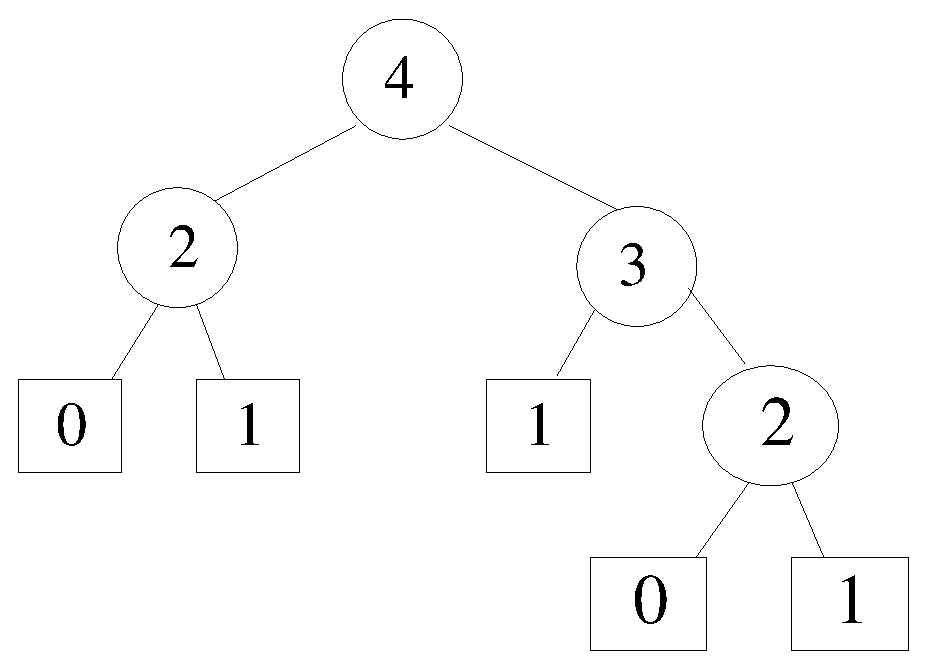
\includegraphics[width=0.7\linewidth]{arbreFibonacci.eps}
\end{center}

\Question{L'arbre de Fibonacci $T_4$ est dessin\'e ci-dessus. $T_0$ est une feuille portant l'\'etiquette 0,
$T_1$ est une feuille portant  l'\'etiquette 1; pour $n>1$, $T_n$ est un noeud binaire, dont le fils gauche est $T_{n-2}$ et dont le fils droit est $T_{n-1}$. Donnez une formule r\'ecursive pour 
le nombre d'\'el\'ements (feuilles ou sommets), not\'e $|T_n|$,  de $T_n$, pour $n>1$}

~\\
~\\



\Question{D\'efinissez $U_n$ le nombre de feuilles \'etiquet\'ees 1 de $T_n$. Que constatez-vous}

~\\
~\\
~\\

\Question{D\'efinissez $Z_n$ le nombre de feuilles \'etiquet\'ees 0 de $T_n$}

~\\
~\\
~\\

\Question{Remplissez le tableau suivant, o\`u $U_n$ est le nombre de feuilles \'etiquet\'ees 1 de $T_n$,
$Z_n$ le nombre de feuilles \'etiquet\'ees 0 de $T_n$}

{\Large
$$
\begin{array}{|c|c|c|c|c|c|c|c|c|c|c|}
\hline
n & 0 & 1 & 2 & 3 & 4 & 5 & 6 & 7 & 8 & 9 \\
\hline
|T_n| & & & & & & & & & &  \\
\hline
U_n & & & & & & & & & &  \\
\hline
Z_n & & & & & & & & & &  \\
\hline
\end{array}
$$
}

\end{multicols}
\end{document}
\Question{Prolongez de fa\c{c}on logique la suite de Fibonacci aux nombres n\'egatifs}
$$\begin{array}{|c|cccccccccccc|}
\hline
i & -6 & -5 & -4 & -3 & -2 & -1 & 0 & 1 & 2 & 3 & 4 & 5  \\
\hline
F_i & & & & & & & 0 & 1 & 1 & 2 & 3 & 5  \\
\hline
\end{array}
$$


\Question{Vous constatez que, pour $n\in \N$,  $F_{-2n}$ est \'egal \`a}

~\\

\Question{Vous constatez que, pour $n\in \N$,  $F_{-2n-1}$ est \'egal \`a}

~\\
 

\Question{ Soient $\phi=\frac{1}{2}(1+\sqrt{5})\approx 1.618$ et $\phi'=\frac{1}{2}(1-\sqrt{5})\approx -0.618$~; ce sont les deux racines de $x^2-x-1=0$. 
D\'efinissons $f(n)=\frac{1}{\sqrt{5}}(\phi^n - \phi'^n)$.
Donnez la valeur de $f(0), f(1), f(2), f(3)$} 

\Question{Par r\'ecurrence, prouvez que $F_n=f(n)$}

~\\
~\\
~\\
~\\
~\\

\Question{Le temps d'ex\'ecution d'un algorithme  est
$T(n)$ pour une donn\'ee de taille $n$, o\`u $T(1)=1$ et $T(n)=3 T(n/2)+n$.
Prouver par r\'ecurrence que $T(2^k) = 3^{k+1}-2^{k+1}$}

~\\
~\\
~\\
~\\
~\\

\Question{Prouvez que $3^{\log_2 n}$ est en $O(n ^{log_3 2})$ (Remarque: $\log_3 2\approx 1.5849625$)}

~\\
~\\
~\\
~\\
~\\


\Question{Calculer le produit scalaire entre 2 vecteurs de $n$ nombres flottants $u=(u_i)$ et $v=(v_i)$ n\'ecessite}
\begin{Reponse}
\Faux $O(\log n)$ op\'erations flottantes
\Vrai $O( n)$ op\'erations flottantes
\Faux $O( n\log n)$ op\'erations flottantes
\Faux $O( n^2)$ op\'erations flottantes
\end{Reponse}

\Question{Calculer le produit entre une matrice carr\'ee quelconque de taille $n\times n$, contenant $n^2$  nombres flottants, et un vecteur colonne de $n$ \'el\'ements ($n$ nombres flottants)
n\'ecessite}
\begin{Reponse}
\Faux $O(n \log n)$ op\'erations flottantes
\Faux  $O(n )$ op\'erations flottantes
\Vrai  $O(n^2 )$ op\'erations flottantes
\Faux ce n'est pas toujours possible
\end{Reponse}

\Question{Calculer le produit entre deux matrices carr\'ees de taille  $n\times n$, en appliquant la formule~: $C_{lc}=\sum_{k=1}^n A_{lk}\times B_{kc}$, n\'ecessite}
\begin{Reponse}
\Faux $O(n \log n)$ op\'erations flottantes
\Faux  $O(n )$ op\'erations flottantes
\Vrai  $O(n^2 )$ op\'erations flottantes
\Vrai  $O(n^3 )$ op\'erations flottantes
\Faux ce n'est pas toujours possible (la matrice doit \^etre inversible, par exemple).
\end{Reponse}

\Question{La m\'ethode de puissance rapide pour calculer $M^k$ ($M$ est une matrice carr\'ee de taille $n\times n$, et $k$ est un entier naturel)  n\'ecessite}  
\begin{Reponse}
\Faux in\'evitablement $k-1$ (donc $O(k)$) multiplications de matrices carr\'ees de taille $n\times n$
\Vrai $O(\log k)$ multiplications de matrices carr\'ees de taille $n\times n$
\Vrai $O(k\log k)$ multiplications de matrices carr\'ees de taille $n\times n$
\Faux ce n'est pas toujours possible (la matrice doit \^etre inversible, par exemple).
\end{Reponse}


\Question{Trouver l'\'el\'ement le plus petit dans une liste non ordonn\'ee de taille $n>0$  n\'ecessite}
\begin{Reponse} 
\Faux $O(1)$ comparaisons
\Faux $O(n^2)$ comparaisons
\Vrai $O(n)$ comparaisons
\Faux $O(\log n)$ comparaisons
\end{Reponse} 

\Question{Trouver l'\'el\'ement le plus petit dans une liste tri\'ee par ordre croissant et de taille $n>0$  n\'ecessite}
\begin{Reponse} 
\Vrai $O(1)$ comparaisons
\Faux $O(n^2)$ comparaisons
\Vrai $O(n)$ comparaisons
\Faux $O(\log n)$ comparaisons
\end{Reponse}


\Question{
Un \'etudiant programme le tri rapide ("quicksort") d'une liste $L$ ainsi~: si $L$  contient moins de 2 \'el\'ements, alors elle est d\'ej\`a tri\'ee. Sinon, l'\'etudiant choisit un \'el\'ement $p$  dans $L$. Il partitionne $L$  
en 3 sous listes, la liste $L_1$ des \'el\'ements dans $L$ inf\'erieurs \`a $p$, la liste $L_2$ des \'el\'ements dans $L$
\'egaux \`a $p$,  
la liste $L_3$  des \'el\'ements dans $L$ sup\'erieurs \`a $p$. Il trie r\'ecursivement les 3 listes, puis concat\`ene les r\'esultats. 
Qu'en pensez-vous}
\begin{Reponse}
\Faux la m\'ethode est correcte mais la complexit\'e est modifi\'ee
\Faux la m\'ethode est correcte et la complexit\'e est inchang\'ee
\Vrai la m\'ethode est incorrecte ; elle boucle quand  $L$ contient deux (ou davantage) \'el\'ements \'egaux \`a $p$.
\Faux la m\'ethode est incorrecte car $L_2$ n'est jamais vide, puisqu'elle contient $p$.
\end{Reponse}


\Question{Pour le calcul de l'arbre couvrant minimum d'un graphe connexe, 
un \'etudiant propose l'algorithme suivant: si le graphe est un arbre, alors ins\'erer cet arbre dans l'arbre couvrant minimum;
sinon d\'ecomposer le graphe $G$ en 2 graphes de taille \`a peu pr\`es moiti\'e, $G_1$, et $G_2$, tous deux connexes; calculer
l'arbre couvrant minimum de $G_1$; calculer l'arbre couvrant minimum de $G_2$; joindre ces deux arbres par l'ar\^ete de co\^ut
 minimum entre $G_1$ et $G_2$ (cette ar\^ete a un sommet dans $G_1$ et un sommet dans $G_2$). 
Que pensez-vous de cet algorithme} 

\begin{Reponse}
\Faux il est correct
\Faux il est difficile de partitionner un graphe connexe en deux sous graphes connexes ayant (\`a peu pr\`es) deux fois moins de sommets; c'est pourquoi cet algorithme n'est pas utilis\'e
\Vrai il est incorrect, et voici un contre exemple simple (au plus 4 sommets!) :

~ \\
 ~ \\
~ \\
~ \\

\end{Reponse}


\Question{Une matrice de Vandermonde a la structure suivante~:
$$M= \left( \begin{array}{ccccc}
1 & 1 & 1 & \ldots & 1 \\
1 & w & w^2 & \ldots & w^{n-1} \\
1 & w^2 & w^4 & \ldots &  w^{2(n-1)} \\
\ldots & \ldots & \ldots & \ldots \\
1 & w^{n-1} &  w^{2n-2} &  \ldots & w^{(n-1)^2} \\
\end{array} \right)
$$ o\`u $n$ est une puissance de 2.
Si de plus $w$ est une racine $n$ i\`eme de l'unit\'e, alors le produit avec un vecteur colonne quelconque de taille $n$}
\begin{Reponse}
\Vrai peut se faire en $O(n \log n)$ (avec l'algorithme de la transform\'ee rapide de Fourier) 
\Vrai ne  peut pas se faire en moins que  $O(n)$
\Faux ne peut pas se faire en moins que $O(n^2)$
\end{Reponse}

\Question{Pour $n=8$ (donc $w^8=1$), \'ecrire la ligne de la matrice de Vandermonde commen\c{c}ant par $1$ puis  $w^3$, en simplifiant
(c'est \`a dire en \'eliminant les puissances plus grandes que 7)}

~\\
~\\
~\\
~\\

\Question{Idem, pour $n=8$, \'ecrire la ligne de la matrice de Vandermonde commen\c{c}ant par $1$ puis  $w^6$}

~\\
~\\
~\\
~\\

\Question{Dans le probl\`eme de la somme, un ensemble $E$ de $n$ entiers positifs $e_1 \ge e_2 \ge \ldots \ge e_n$ est donn\'e, ainsi
qu'un entier $0<S < \sum_1^n e_i$. Il faut trouver le sous ensemble $X$ de $E$ dont la somme des \'el\'ements
est maximum, mais inf\'erieure ou \'egale \`a $S$.  Pour tout ensemble $K$, on note $\sigma(K)$ la somme des \'el\'ements de $K$.
L'algorithme glouton calcule $X_0=\emptyset$ (donc $s(X_0)=0$);  puis, 
pour $i$ de 1 \`a $n$, il calcule $X_i= X_{i-1} \cup \{e_i\}$ si $e_i + \sigma(X_{i-1}) \le S$, et
$X_i= X_{i-1}$ sinon. Avec $E=100,25,20,10,1,1,1$ et $S=40$, donnez les valeurs de $X_0, X_1, \ldots X_7$, et les $\sigma(X_i)$ correspondants}

~\\
~\\
~\\
~\\
~\\
~\\
~\\

\Question{
Cet algorithme donne-t-il un sous ensemble $X_n$}
\begin{Reponse} 
\Vrai toujours correct ($s(X_n)\le S$), mais pas forc\'ement optimal : donnez un exemple simple ($n<5$) o\`u $X_n$ n'est pas optimal\\
~
\Faux toujours correct, et toujours optimal
\Faux pas toujours correct, mais optimal :  donnez un exemple simple ($n<5$) \\
~ 
\Faux souvent correct, et souvent optimal
\Faux ni correct ni optimal : donnez un exemple simple ($n<5$) \\
~
\Faux toutes les r\'eponses pr\'ec\'edentes sont fausses 
\end{Reponse}


\Question{Arthur conjecture que si, dans un graphe non orient\'e, tous les sommets distincts soit sont voisins, 
soit ont un voisin en commun, alors il existe au moins un sommet qui est voisin de tous les autres.  Que pensez vous de cette conjecture}
\begin{Reponse}
\Faux elle est vraie
\Vrai elle est fausse et vous en dessinez un contre exemple simple \\
~\\
\end{Reponse}


\end{multicols}
\end{document}
